%%%%%%%%%%%%%%%%%% Automated attack generation against KF + chi-square %%%%%%%%%%%%%%%%%%%%%%%%%%%
Consider the attacked measurement model
\begin{equation}\label{equ:adversarial_measurement_model}
\mathbf{y}_i^a=C\mathbf{x}_i^a+\mathbf{v}_i+\mathbf{e}_i,
\end{equation}
where $\mathbf{e}_i\in\mathbb{R}^m$ is $k$-sparse. Superscripts $a$ and $0$ denote attacked and nominal closed-loop trajectories driven by identical realizations of the process and measurement noises. The analysis considers deterministic attacks that are independent of these noises and begin at the left endpoint of the detection window. The objective of the attack generator is to produce sequences that significantly perturb a critical output while remaining difficult to detect using \eqref{equ:chisq_detector}.

\subsection{Attack-induced innovation and output maps}
The discriminator construction is developed for the steady-state Kalman gain $K$. Define
\[
\delta\mathbf{x}_i=\mathbf{x}_i^a-\mathbf{x}_i^0,\qquad
\delta\hat{\mathbf{x}}_{i|i-1}
=\hat{\mathbf{x}}_{i|i-1}^a-\hat{\mathbf{x}}_{i|i-1}^0,
\]
and let $\boldsymbol{\zeta}_i=\operatorname{col}(\delta\mathbf{x}_i,
\delta\hat{\mathbf{x}}_{i|i-1})$. The attack-induced innovation is
\begin{equation}\label{equ:innovation_attack}
\delta\mathbf{r}_i
=\mathbf{r}_i^a-\mathbf{r}_i^0
=D\boldsymbol{\zeta}_i+\mathbf{e}_i,\qquad
D=\begin{bmatrix}C&-C\end{bmatrix}.
\end{equation}
Under the control law \eqref{equ:controller}, direct substitution of the KF update gives the augmented recursion
\begin{equation}\label{equ:augmented_attack_map}
\boldsymbol{\zeta}_{i+1}=F_a\boldsymbol{\zeta}_i+G_a\mathbf{e}_i,
\end{equation}
where, with $A_c=A+BK_p$,
\begin{align}
F_a&=
\begin{bmatrix}
A+BK_pKC & BK_p(I-KC)\\
A_cKC & A_c(I-KC)
\end{bmatrix}, \nonumber\\
G_a&=
\begin{bmatrix}
BK_pK\\ A_cK
\end{bmatrix}. \label{equ:FaGa}
\end{align}
Equations \eqref{equ:innovation_attack}--\eqref{equ:FaGa} account for the propagation of earlier attacks through both the plant and the estimator. For a window $\mathcal I=[i-T+1,i]$ and zero attack-induced deviation at its beginning, unrolling these equations yields
\begin{equation}\label{equ:M2}
\delta\mathbf{r}_{\mathcal I}=\mathcal{H}_r\mathbf{e}_{\mathcal I},\qquad
M_2=\operatorname{blkdiag}(S^{-1/2},\ldots,S^{-1/2})\mathcal{H}_r,
\end{equation}
where $\mathcal{H}_r$ is block lower triangular, with identity diagonal blocks and subdiagonal block $(p,q)$ equal to $DF_a^{p-q-1}G_a$ for $p>q$.

Let $\mathbf{y}_{c,i}=C_c\mathbf{x}_i$ denote the critical output. The corresponding stacked perturbation satisfies
\begin{equation}\label{equ:M1}
\delta\mathbf{y}_{c,\mathcal I}=\mathcal{H}_c\mathbf{e}_{\mathcal I}
\triangleq M_1\mathbf{e}_{\mathcal I},
\end{equation}
where $\mathcal{H}_c$ is obtained by unrolling \eqref{equ:augmented_attack_map} with output matrix $\begin{bmatrix}C_c&0\end{bmatrix}$. Thus $M_1$ captures the complete plant--controller--estimator response, whereas $M_2$ captures the complete normalized innovation response.

\subsection{Successful attacks and generative model}
Under the deterministic, noise-independent, window-initialized attack model stated above, the windowed statistic has the noncentral chi-square distribution
\begin{equation}\label{equ:noncentral_chisq}
g_{\mathcal I}^a\sim\chi_{Tm}^{\prime 2}(\lambda_{\mathcal I}),\qquad
\lambda_{\mathcal I}=\|M_2\mathbf{e}_{\mathcal I}\|_2^2.
\end{equation}
Accordingly, $\lambda_{\mathcal I}$ determines the detection probability
\begin{equation}\label{equ:detection_probability}
P_D(\mathbf{e}_{\mathcal I})
=1-F_{\chi_{Tm}^{\prime 2}(\lambda_{\mathcal I})}
\big(\tau_{\chi^2,\mathcal I}(\beta)\big),
\end{equation}
where $\tau_{\chi^2,\mathcal I}(\beta)=F_{\chi^2_{Tm}}^{-1}(1-\beta)$.

\begin{definition}[$(\alpha,\gamma)$-successful FDIA]\label{Def:Successful_FDIA}
Define the per-time sparsity set
\[
\Sigma_k^{(T)}=\{\mathbf{e}_{\mathcal I}:
\|\mathbf{e}_j\|_0\le k,\ j\in\mathcal I\}.
\]
An attack sequence $\mathbf{e}_{\mathcal I}\in\Sigma_k^{(T)}$ is $(\alpha,\gamma)$-successful if
\begin{equation}\label{equ:def_success_FDIA}
\|M_1\mathbf{e}_{\mathcal I}\|_2\ge\alpha,
\qquad
P_D(\mathbf{e}_{\mathcal I})\le\gamma,
\end{equation}
where $\alpha>0$ is the required critical-output perturbation and $\gamma\in(\beta,1)$ is the maximum admissible detection probability.
\end{definition}
Because \eqref{equ:detection_probability} is monotone in $\lambda_{\mathcal I}$, the second condition is equivalently represented by
\begin{equation}\label{equ:lambda_max}
\|M_2\mathbf{e}_{\mathcal I}\|_2^2\le\lambda_{\max}(\beta,\gamma),
\end{equation}
where $\lambda_{\max}$ is the unique noncentrality level that yields $P_D=\gamma$. This replaces an ad hoc residual threshold with a detector-calibrated stealthiness constraint.

The feasible attack set is therefore
\begin{equation}\label{equ:success_FDIA_set}
\begin{aligned}
\mathcal{S}(\alpha,\gamma)=\{\mathbf{e}\in\Sigma_k^{(T)}:\ &
\|M_1\mathbf{e}\|_2\ge\alpha,\\
&\|M_2\mathbf{e}\|_2^2\le\lambda_{\max}(\beta,\gamma)\}.
\end{aligned}
\end{equation}
We approximate this set using a neural generator $G(\mathbf{z};\boldsymbol{\theta}_g)$, with $\mathbf{z}\sim P_z$. Let $\Pi_{k,T}$ retain the $k$ largest-magnitude entries in each time block and set all other entries to zero. The generated attack is defined as
\begin{equation}\label{equ:sparse_generator}
\mathbf{e}_{\mathcal I}=\Pi_{k,T}\!\left(G(\mathbf{z};\boldsymbol{\theta}_g)\right),
\end{equation}
which enforces membership in $\Sigma_k^{(T)}$. The plant and filter maps $M_1$ and $M_2$ act as fixed physics-based discriminators, as illustrated in Fig.~\ref{fig:GM}.

\begin{figure}[h!]
    \centering
    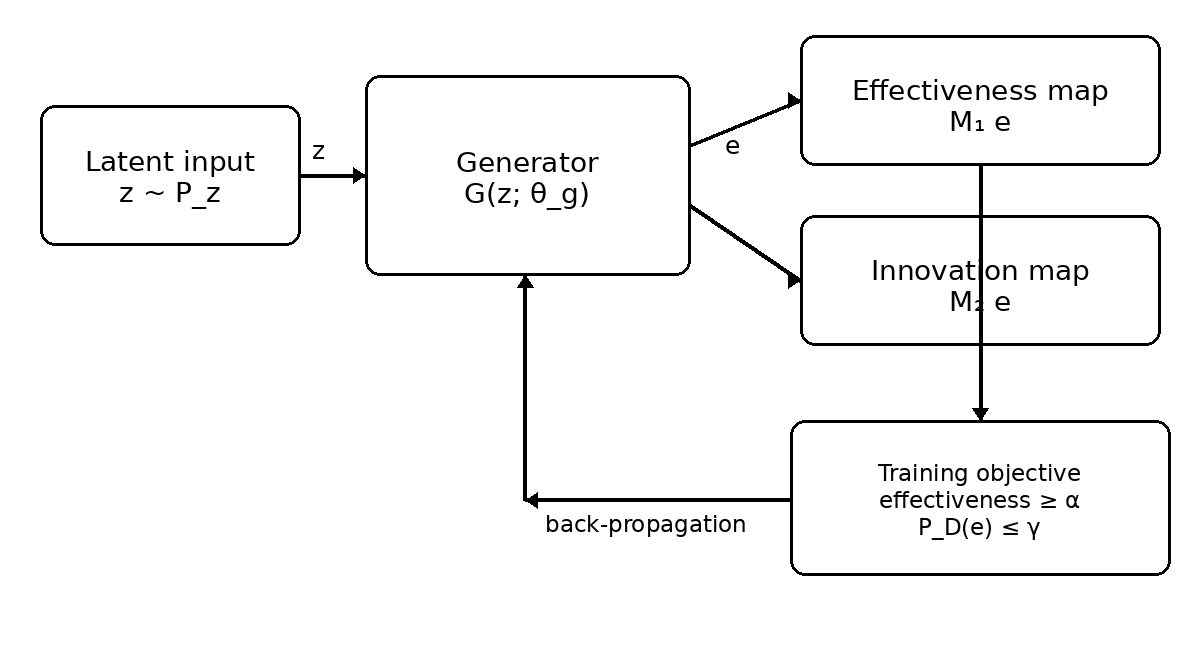
\includegraphics[width=\columnwidth]{image/GM.png}
    \caption{Physics-guided attack generation. The discriminator $M_1$ evaluates critical-output effectiveness, whereas $M_2$ determines the noncentrality parameter of the windowed chi-square detector.}
    \label{fig:GM}
\end{figure}

The generator is trained using
\begin{align}
J(\mathbf{e})={}&
\operatorname{ReLU}\!\left(\alpha-\|M_1\mathbf{e}\|_2\right)\nonumber\\
&+\operatorname{ReLU}\!\left(
\|M_2\mathbf{e}\|_2^2-\lambda_{\max}(\beta,\gamma)
\right), \label{equ:generator_loss}\\
\boldsymbol{\theta}_g^\star
={}&\argmin_{\boldsymbol{\theta}_g}
\mathbb{E}_{\mathbf{z}\sim P_z}
\left[J\!\left(\Pi_{k,T}(G(\mathbf{z};\boldsymbol{\theta}_g))\right)\right].
\label{equ:training_GM}
\end{align}
The resulting labeled samples are used to train the channel-wise localization model in Section~\ref{sec:detection_localization}.
